\setchapterpreamble[u]{\margintoc}
\chapter{Consistent Mass-Momentum Transport}
\labch{momcons}

% intro : PARIS Simulator, necessity due to large density-ratios ? 

The stability of numerical methods that attempt to model 
interfacial flows involving large density contrasts 
face several challenges, key amongst them being the transport of 
mathematical discontinuities that arise from the contrast in
the material properties of the fluids involved. 
Extremely small numerical errors are ubiquitous as a consequence of the 
numerous approximations involved at each and every step of the algorithm 
In the context of such flows, such errors generally result in physically
inconsistent mass and momentum transfer across the interface, often from
the denser phase towards the lighter phase.
The presence of large density or viscosity contrasts tend to amplify
the growth of these cascading numerical errors, eventually
leading to significant (often catastrophic) interfacial deformations
followed rapidly by a loss of numerical stability. 
In this chapter, we present a detailed exposition of our class 
of numerical methods which are designed specifically to circumvent or
suppress the growth of such numerical instabilities when dealing with
flows entailing large density-ratios. 
The implementations of the numerical algorithms are developed for 
finite volume discretizations using uniform Cartesian grids in 3D, 
on the `PARIS Simulator' \cite{paris} numerical platform.      

% ----------------------------------------------------------------------------------------------------------------------

\section{General Principles}

%intro : what do you mean by consistent transport? 
In the past two decades, considerable efforts have been made 
in the design of numerical methods to deal with marked density contrasts
\sidenote{By marked density contrasts, we mean large $|\log r|$, where $r$ 
is the ratio of the densities of the two fluids.}. 
The underlying principle behind these endeavours is that the governing 
equations for the transport of mass and momentum are modeled using a 
conservative formulation (divergence of fluxes), instead of standard 
non-conservative forms which themselves were adapted directly from 
techniques developed originally for single-phase flows. 
This formulation enables one to render the discrete transport of 
momentum \textit{consistent} with respect to the discrete transport of mass  
Such a tight coupling of the propagation of errors between the discrete 
mass and momentum fields enables alleviation of many of the issues 
that plague such numerical methods, especially in the 
context of low to moderate spatial resolutions. 
A secondary but important mitigating factor is the advancements 
made in the modeling of capillary forces, resulting in the adoption of 
consistent and \textit{well-balanced} surface tension formulations.
\sidenote{Consistency in the context of surface tension models refers to the ability 
of methods to progressively achieve more accurate estimations of interfacial 
curvature as a result of increasing spatial resolution, 
whereas well-balanced refers to the ability to recover certain static 
equilibrium solutions pertaining to surface tension dominated flows 
without the perpetual presence of parasitic or spurious currents in the velocity fields.}.
We refer the reader to influential works of Popinet \cite{popinet2018numerical,popinet2009accurate}
to get a better understanding of the issues surrounding surface tension implementations.  

\subsection*{Major Iterations in Literature}

% literature review 

% Rudman (1998) :
The first study to address the issue of consistency between mass 
and momentum transport was the seminal work of Rudman \sidecite{rudman1998volume}.
The fundamental hurdle in the implementation of mass-momentum 
consistent transport for staggered configurations of primary variables 
(pressure and velocity) is the inherent difficulty in reconstructing mass 
(defined on centered control volumes) and its corresponding fluxes 
onto the staggered control volumes on which momentum is defined. 
Rudman introduced the strategy of carrying out mass advection 
\sidenote{Mass advection was carried out using using algebraic flux reconstructions.} 
on a grid twice as fine as that of momentum, 
thereby enabling a `natural' and intutive 
way to reconstruct mass and its fluxes onto staggered momentum control volumes. 
However, their method uses a VOF based convolution technique for curvature computation, 
which is neither consistent nor well-balanced.    


% Bussmann et al. (2002) :
Bussmann et al. \sidecite{bussmann2002modeling} were able to 
circumvent the issue surrounding staggered grids altogether 
by using a collocated arrangement in the context of hexahedral 
unstructured meshes, coupled with an unsplit Eulerian flux computation method.    
The study though makes no mention of any surface tension model. 


% Raessi & Pitsch (2012) | Ghods & Hermann (2013):
Level set based methods in the context of mass-momentum consistent 
transport were implemented first by Raessi and Pitsch \sidecite{raessi2012consistent}, 
followed by Ghods and Hermann \cite{ghods2013consistent}. 
In the former, the consistency problem is tackled by means of a 
semi-Lagrangian approach, computing geometric level set derived 
fluxes at two different time intervals, whereas in the latter, 
a collocated arrangement is used. 
Nonetheless, both methods face certain drawbacks, notably the 
applicability only to 2D in case of Raessi and Pitsch, 
as well as a lack of well-balanced surface tension models for both these methods.   


% LeChenadec & Pitsch (2013) | Owkes & Desjardins (2017) : 
Recent advances concerning volume-of-fluid based methods that 
employ unsplit (conservative) geometric flux reconstructions 
were made by LeChenadec and Pitsch \sidecite{le2013monotonicity}
, and later by Owkes and Desjardins \cite{owkes2017mass}. 
LeChenadec and Pitsch utilize a Lagrangian remap method in order 
to construct consistent mass-momentum fluxes for the staggered control volumes, 
while Owkes and Desjardins use mass advection on a doubly refined grid 
(same principle as Rudman) to achieve consistency.     
Although \cite{le2013monotonicity} implements a well-balanced surface tension model, 
the VOF convolution based curvature computation is not consistent. 
In case of \sidecite{owkes2017mass}, they use mesh-decoupled height functions 
to compute curvature while coupling it with a well-balanced surface tension model. 
However, their semi-Lagrangian flux computation procedure 
involving streak tubes and flux polyhedra are extremely convoluted in 3D.     


% Vaudor et al. (2017) | Zuzio et al. (2020) : 
Certain methods attempt to combine the qualities of both 
VOF and level set methodologies (CLSVOF), as proposed in the works of 
Vaudor et al. \sidecite{vaudor2017consistent}, 
and more recently by Zuzio et al. \cite{zuzio2020new}. 
They both tackle the consistency issue by means of projecting 
the direction-split geometric fluxes onto a twice finer grid, 
which are subsequently recombined to reconstruct consistent 
fluxes for mass and momentum for the staggered control volumes. 
This approach allows them to bypass the requirement of conducting 
mass advection on a twice finer grid (as in the original Rudman method), 
thereby deriving the benefits of a sub grid without the 
added computational cost of doubly refined mass transport. 
In addition, both Vaudor et al. \cite{vaudor2017consistent} and 
Zuzio et al. \sidecite{zuzio2020new} adopt well-balanced surface tension 
models with consistent level set based curvature estimation. 
However, the purported advantages of both these methods with 
regard to reduced computational costs is not quite evident, 
as additional complexities are introduced due to the projection 
(reconstruction) of fluxes onto a the twice finer mesh, 
which would not be necessary in the first place if mass transport 
had been carried out on the twice finer mesh itself. 


% Patel & Natarajan (2017) : 
Patel and Natarajan \sidecite{patel2017novel} developed a hybrid 
staggered-collocated approach to solve the consistency issue on 
polygonal unstructured meshes, complemented with a well-balanced surface tension model. 
Nevertheless, the VOF advection is based on algebraic transport, 
not to mention the use of a VOF convolution based 
curvature computation, which is inherently not consistent. 


% Nangia et el. (2019) : 
More recently, Nangia et al. \sidecite{nangia2019robust} developed a 
CSLVOF method for dynamically refined staggered Cartesian grids. 
They utilize Cubic Upwind Interpolation (CUI) schemes to 
reconstruct consistent mass and momentum fluxes on the staggered 
control volumes, using the information from the additional mass 
advection equation they solve alongside the level set function.   
However, the reconstruction of mass fluxes using CUI schemes are 
inherently algebraic, with their comparative advantage against fluxes 
computed via geometric constructions being an open question 
\sidenote{refer to Mirjalili et al. \cite{mirjalili2017interface}. }.

To get a bird's eye view of the numerous features employed by the methods 
in existing literature, we refer the reader to tables %\ref{table_vof} and \ref{table_ls}, 
which respectively provide systematic overviews of the VOF based and level set based approaches.    

% modified comparison charts with CAF paper added



\subsection*{Our Approach}

In the present body of work, we start by precisely defining the
essential (desired) attributes of a numerical scheme that 
ensures discrete consistency between mass and momentum transport : 

\begin{itemize}
	\item The discontinuity of the mass (volume fraction 
		derived density field) should propagate at the 
		exact `numerical' speed as that of 
		the discontinuity of the momentum field. 
	\item The numerical transport of momentum should be performed 
		in a manner consistent with the transport of mass for 
		each direction, implying that the momentum fluxes must 
		be obtained directly from geometrically 
		computed fluxes of mass (volume). 
\end{itemize}

In order to tackle the challenge of consistent transport on staggered control 
\sidenote{`PARIS Simulator' has a staggered configuration of primitive 
variables on regular Cartesian control volumes.}
volume configurations, we have developed two different strategies, namely, 
the \textit{shifted fractions} method and the \textit{sub-grid} method. 
The former uses geometrical reconstructions to derive a 
\textit{shifted} volume fraction field which is centered on the staggered
control volumes, whereas the latter adopts the Rudman \cite{rudman1998volume} 
strategy of volume advection on a twice finer grid in order to 
enable consistent reconstruction of mass and momentum on the staggered control volumes. 
Another key contribution of this body of work is to extend the conservative 
direction-split mass transport algorithm of Weymouth and Yue \sidecite{wy} 
to the direction-split transport of momentum. 

A thorough description of the shifted fractions method is can be found in
the recent study by Fuster et al. \sidecite{caf_momcons} 
, and a detailed exposition of the
sub-grid method is currently under preparation at the time of writing.  
We shall be taking a closer look at these two stratetgies in the upcoming sections.  


% ----------------------------------------------------------------------------------------------------------------------


\section{Basic Expressions}

% intro : interfacial propagation 

\newcommand{\dert}[1]{\frac{\partial #1}{\partial t}}
\newcommand{\cijk}{C_{i,j,k}}
\newcommand{\pijk}{\phi_{i,j,k}}
\newcommand{\X}{\boldsymbol{x}}
\newcommand{\N}{\boldsymbol{n}}
\newcommand{\rijk}{\rho_{i,j,k}}
\newcommand\mijk{(\rho u_{q})_{i,j,k}}

We start with the advection of the interface position, which in 
the VOF framework is given by - 

\marginnote{In the VOF approach, the approximation to the interface Heaviside 
function contains a sharp discontinuity, in contrast to the level set approach 
where the approximation is continuous in the discrete sense.}


\begin{align}
	\dert H + \nabla \cdot (\boldsymbol{u} H) = H\, \left(\nabla \cdot \boldsymbol{u} \right) \,
	\label{heaviside}
\end{align}


Integrating this equation in time after carrying 
out spatial discretization, one obtains -    


\marginnote{$\cijk^n$ is the colour function or volume fraction field at time step $n$ 
obtained through the finite volume discretization of the interface Heaviside function.}


\begin{align}
{\cijk^{n+1} - \cijk^{n}} = - \sum_{\textrm{faces} \, f} F^{(c)}_f + \int_{t_n}^{t_{n+1}}  
	{\textrm{d}}t \int_\Omega  H \, \left(\nabla \cdot \boldsymbol{u}\right) \,  {\textrm {d}}\X   \,,
\label{sumf}
\end{align}


where the first term on the right-hand side is the summation over the cell faces $f$  
of the fluxes $F^{(c)}_f$   
\sidenote{These fluxes of $(\boldsymbol{u} H)$ are computed via geometrical reconstructions,
and not via high-order non-linear interpolation schemes which are 
the standard (in the absence of discontinuities) . } . 
As one can clearly observe, the ``compression'' term on the 
right-hand side of equation \eqref{heaviside} disappears for incompressible flow, 
however it is essential in the context of direction-split geometric advection schemes.
The definition of the geometric fluxes in mathematical form is -  

\begin{align}
	F_f^{(c)} = \int_{t_n}^{t_{n+1}} {\textrm {d}}t \int_{f} u_f(\X,t) H(\X,t) \, {\textrm{d}}\X \,,
\label{faceint}
\end{align}

where $u_f = \boldsymbol{u}\cdot \N_f$ 
\sidenote{Component of the velocity normal to the control surface $f$.}.
Once an approximation for the evolution of $(\boldsymbol{u} H)$ during
the time step is chosen, a four-dimensional integral remains to be
computed in equation (\ref{faceint}).
The advection schemes used are CIAM and Weymouth-Yue, which have been 
described briefly in chapter \ref{ch:method}. 

Directional splitting results in the breakdown of equation (\ref{sumf}) 
into three equations, one for each advection substep -


\begin{align}
{\cijk^{n,l+1} - \cijk^{n,l}} = - F^{(c)}_{m-} - F^{(c)}_{m+} 
+ c_m \partial_{m}^h u_m \,,
\label{sumf2}
\end{align}


\marginnote{The superscript $l=0,1,2$ is the substep index, i.e.
$\cijk^{n,0} = \cijk^{n}$ and $\cijk^{n,3} = \cijk^{n+1}$. 
The face with subscript $m-$ is the ``left'' face in direction $m$ with 
$F^{(c)}_{m-} \ge 0$ if the flow is locally from right to left. A similar reasoning 
applies to the ``right'' face $m+$.}

After each advection substep (\ref{sumf2}), the interface is reconstructed
with the updated volumes $\cijk^{n,l+1}$, then the 
fluxes $F^{(c)}_{f}$ are computed for the next substep. 
Importantly, we have approximated the compression term in (\ref{sumf}) by -

\begin{align}
	\int_{t_n}^{t_{n+1}}  {\textrm {d}}t \int_\Omega  H \partial_m u_m  {\textrm {d}}\X \simeq  c_m 
 \partial_{m}^h u_m \, 
 \label{comp}
\end{align}

\marginnote{There is no implicit summation carried out 
over $m$, and the superscript $h$
denotes the spatial discretization of the operator. } 

On the right hand sides of (\ref{sumf2}) and (\ref{comp}) 
the flux terms $F_{f}^{(c)}$ and the 
 partial derivative $\partial_{m} u_m$ must
be evaluated using identical discretized velocities.
The expression $\partial_{m}^h u_m$ is a finite volume approximation of the 
spatial derivative corresponding to the $m$th component 
of the velocity vector along direction $m$, and
the ``compression coefficient'' $c_m$ approximates the color fraction. 
Its exact expression is dependent on the advection method
\sidenote{Refer to chapter \ref{ch:method} to see the difference in
the definitions of the compression coefficient between  
the CIAM and Weymouth-Yue methods.}
and it also entails the desirable property of $C$-bracketing
\sidenote{The preservation of $0 \le \cijk \le 1$ 
is referred to as $C$-bracketing. }. 
Due to the possible dependence of the 
compression coefficient $c_m$ on the Cartesian direction
corresponding to the advection substep, 
the sum $\sum_m c_m \partial_{m}^h u_m$ may not necessarily vanish
even if the flow is incompressible.
As mentioned previously in chapter \ref{ch:method}, the main appeal
of the Weymouth-Yue method is its ability to keep this sum to zero,
within the limits of machine precision. 

\subsection*{Advection of Conserved Scalars}  

In order to achieve consistent transport of the discontinuous fields 
of mass and momentum, we start by trying to understand the advection 
of a generic \textit{conserved} scalar quantity $\phi$ by a continuous velocity field - 


\begin{align}
	\dert \phi + \nabla \cdot \left( \phi \, \boldsymbol{u} \right)  = 0 
\label{phiconv}
\end{align}


where the field $\phi$ is smoothly varying except 
at the interface position, where it may be discontinuous.
The essence of this study lies in the search of a scheme that  
propagates this discontinuity ($\phi$) at the same speed as 
that of the advection of volume fraction ($C$).

\marginnote{The smoothness of the advected quantity away from the interface
is verified for fields such as density $\rho$, momentum $\rho \boldsymbol{u}$ 
and internal energy $\rho e$.}

Temporal integration of the spatially discretized version of \eqref{phiconv} gives us - 

\begin{align}
\pijk^{n+1} - \pijk^{n} = - \sum_{\textrm{faces}\, f} F^{(\phi)}_f 
\label{sumfp}
\end{align}

\marginnote{The sum on the right-hand side is the sum over faces $f$ of cell $i,j,k$ 
of the fluxes $F^{(\phi)}_f$ of $\phi$, which are defined as the color function fluxes
$F^{(c)}_f$ in \eqref{faceint}.}


where the fluxes are defined as -

\begin{align}
	F_f^{(\phi)} = \int_{t_n}^{t_{n+1}} {\textrm {d}}t \int_{f} u_f(\X,t) \,\phi(\X,t) \,
	{\textrm {d}}\X
\label{pfaceint}
\end{align}

In order to ``extract'' the discontinuity we introduce the 
 interface Heaviside function $ H(\X,t) $

\begin{align}
F_f^{(\phi)} = 
\int_{t_n}^{t_{n+1}} {\textrm d}t \int_{f} \left[ u_f  \,H \,\phi  +  u_f \,(1-H) \,\phi \right] 
\, {\textrm d}\X \, 
\label{fluxphi}
\end{align}

Therefore, the flux can be decomposed into two components as -

\begin{align}
F_f^{(\phi)} = 
\bar \phi_1 \int_{t_n}^{t_{n+1}} {\textrm d}t \int_{f} u_f \,H \,{\textrm d}\X + 
\bar \phi_2 \int_{t_n}^{t_{n+1}} {\textrm d}t \int_{f} u_f \,(1-H) \,{\textrm d}\X \,,
\label{barphi}
\end{align}

where the face averages $\bar \phi_s$, $s=1,2$, are defined as - 


\begin{align} 
\bar \phi_s = \frac{\int_{t_n}^{t_{n+1}} {\textrm d}t \int_{f} \phi \,u_f \,H_s  
{\textrm d}\X}{\int_{t_n}^{t_{n+1}} {\textrm d}t \int_{f}  
u_f \,H_s\,{\textrm d}\X} \,,  
\label{barphi2}
\end{align}


and $H_1=H$, $H_2= 1-H$. 
The total flux can be rearranged as a sum of the constituents 
corresponding to the different `fluids' - 

\marginnote{Expression \eqref{barphi} can be written in terms 
of the fluxes $F^{(c)}_f$ and $F^{(1-c)}_f$, this second one being obtained by 
replacing $H$ with $1-H$ in \eqref{faceint}}

\begin{align}
F_f^{(\phi)} = \bar \phi_1 \,F_f^{(c)} +  \bar \phi_2 \,F_f^{(1-c)} \,.
\label{fluxphi12}
\end{align}



\subsection*{Advection of Density}
% VOF - rho consistency with compression term etc

The density field $\rho(\X,t)$ follows the 
temporal evolution of the generic conserved quantity
(\ref{phiconv}) by setting $\phi = \rho$. 
At the incompressible limit the velocity field is 
solenoidal (divergence-free), with constant densities 
in each phase. We can extract the density trivially from the integrals 
\eqref{barphi2} to \textit{exactly} obtain $\bar \rho_s = \rho_s$. 
The flux definitions corresponding to $\rho$ become    


\begin{align}
F_f^{(\rho)} = \rho_1 F_f^{(c)} +  \rho_2 F_f^{(1-c)}
\label{fluxrho}
\end{align}

\marginnote{We use the term `conservative' to express the fact
that eq. (\ref{sumfp}) computes the temporal evolution of $\rho$ 
as a difference of fluxes, instead of velocity times its gradient.}


Using the above definitions for density fluxes,
one can employ any VOF method to construct fluxes of the color 
function in order to obtain conservative transport for $\rho$
In principle, this should result in the conservation of total mass.  
However, as we have already pointed out the fact that the CIAM
method does not conserve volume exactly 
\sidenote{This again comes back to the dependence of the compression 
coefficient on the volume fraction field at the start of each
advection substep.}
, consequently, the advection of the density field (mass) 
is not consistent with that of the advection of $C$. 

This apparent paradox is resolved by including the 
compression term on the right hand side of \eqref{phiconv},
in order to ensure consistency. 
The advection equation for the conserved quantity now becomes - 


\begin{align}
\dert \phi + \nabla \cdot ( \phi \,\boldsymbol{u})  = \phi \, \left(\nabla \cdot \boldsymbol{u}\right) 
\label{phiconv2}
\end{align}


This equation can be decomposed into advection substeps corresponding to 
the direction-split integration framework as follows - 

\marginnote{The direction-split integration steps operations for $\phi$
mirror that of the volume fraction $C$. }


\begin{align}
{\pijk^{n,l+1} - \pijk^{n,l}} = - F^{(\phi)}_{m-} - F^{(\phi)}_{m+} 
+ \Big( \tilde \phi_1^m c^{(1)}_m + \tilde \phi_2^m c^{(2)}_m \Big) \, \partial_{m}^h u_m 
\label{sumfpconsistent}
\end{align}


\marginnote{$c^{(1)}_m=c_m$ is the compression coefficient corresponding 
to the particular VOF advection method for volume fraction $C$ ,
while $c^{(2)}_m= 1 -c_m$ corresponds to that of the 
symmetric color fraction  $1 - C$.}


The fluxes $F^{(\phi)}_{m\pm}$ follow the definition given in \eqref{fluxphi12}, 
, while the cell averages $\tilde \phi_s^m$ are defined as - 


\begin{align}
\tilde \phi_s^m = \frac{\int_{t_n}^{t_{n+1}} {\textrm{d}}t \int_{\Omega}  \phi  H_s  
\partial_{m}^h u_m  \,  {\textrm{d}}\X}
{\int_{t_n}^{t_{n+1}} {\textrm{d}}t \int_{\Omega} H_s  \partial_{m}^h u_m \,{\textrm{d}}\X} \,
\label{cellphi2}
\end{align}


Rewriting the direction-split integration operation for $\rho$ we get - 


\marginnote{In case of CIAM, the compression coefficient is defined as
$c_m = \cijk^{n,l}$, whereas in Weymouth-Yue the coefficient is independent
of the advection substep $l$, defined as  
$c_m = H\left(\cijk^{n} - 1/2 \right)$, where $H$ is the Heaviside function.}


\begin{align}
{\rijk^{n,l+1} - \rijk^{n,l}} = - F^{(\rho)}_{m-} - F^{(\rho)}_{m+} + C_m^{(\rho)}\,,
\label{sumfrho}
\end{align}


where the fluxes are given by (\ref{fluxrho}) and the compression term is

\marginnote{Again, there is no implicit summation rule on $m$.} 


\begin{align}
C_m^{(\rho)} =  \left( \rho_1 c^{(1)}_m + \rho_2 c^{(2)}_m \right) \,\partial_{m}^h u_m  
\label{central}
\end{align}



For the WY method, the compression terms eventually cancel upon 
summation over the substeps, therefore resulting in the conservation  
of mass at the same accuracy as the discrete incompressibility condition
$\sum_{m=1}^3 \partial_{m}^h u_m=0$ is verified 
\sidenote{This usually corresponds to the tolerance of the Poisson solver,
with a typical value being $10^{-6}$. }. 



\subsection*{Advection of Momentum}
% model of computing consistent mass-momentum fluxes

Within the framework of advection of a generic conserved scalar,
we consider momentum advection as transport of the scalar quantities  
$\phi=\rho u_q$, where $q=1,2,3$ is the component index. 
Using the definition given in \eqref{barphi2}, 
we obtain the expression -  

\marginnote{The expressions with the `bar' 
refer to face weighted averages of the varible in question. 
Here, $\bar \phi_s = \overline { \rho u_q}_s$ }


\begin{align} 
\overline{\rho u_q}_s = \rho_s \bar u_{q,s} 
\end{align}


where $\bar u_{q,s}$ is termed as the ``advected interpolated velocity'', 
whose precise definition is given as - 


\begin{align}
	\bar u_{q,s} =  \frac{\int_{t_n}^{t_{n+1}} {\textrm{d}}t \int_{f}  u_q u_f  H_s  \, {\textrm{d}}\X}{\int_{t_n}^{t_{n+1}} {\textrm{d}}t \int_{f}  u_f  H_s\,{\textrm{d}}\X} \label{barudef}
\end{align}

\marginnote{The subscript $s$ denotes the phase or fluid,
and $f$ represents the normal components defined on the face
centers.} 


Thus, the direction-split integration of the momentum can be represented as - 


\begin{align}
{\mijk^{n,l+1} - \mijk^{n,l}}  = - F^{(\rho u)}_{m-} - F^{(\rho u)}_{m+}
 + \Big( \rho_1 \tilde u_{q,1}^m  c^{(1)}_m +  \rho_2 \tilde u_{q,2}^m c^{(2)}_m 
 \Big) \, \partial_{m}^h u_m 
\label{sumfrou}
\end{align}


where the momentum fluxes are constructed in the following manner -


\begin{align}
 F^{(\rho u)}_{f} =  \rho_1 \,\bar u_{q,1}  \,F^{(c)}_{f}  +  
 \rho_2 \,\bar u_{q,2}  \,F^{(1-c)}_{f} \,,
\end{align}


The expression for the ``central interpolated velocity'' corresponding to the 
averages $\tilde \phi_s^m$ of \eqref{cellphi2} is -  

\marginnote{Notice that ``cloning'' the advected velocities 
$\bar u_{q,1}$ and $\bar u_{q,2}$ 
would make it easier to advect a velocity field 
with a jump on the interface, but would 
render the overall algorithm quite complicated. }


\begin{align}
	\tilde u_{q,s}^{m} = \frac{\int_{t_n}^{t_{n+1}} {\textrm{d}}t \int_{\Omega} u_q \, H_s \,  
	\partial_{m}^h u_m   \,  {\textrm{d}}\X}
	{\int_{t_n}^{t_{n+1}} {\textrm{d}}t \int_{\Omega} H_s \, \partial_{m}^h u_m \,{\textrm{d}}\X} 
\label{tildeudef}
\end{align}


The superscript $m$ is intentionally omitted  
for the velocities $\tilde u_q^m$ in order to avoid
cumbersome and complicated notations. 

\marginnote{Due to the viscous effects and 
the absence of phase change in our fluid dynamics model,   
the velocity filed maintains continuity across the interface.} 

As a reasonable approximation we choose to put 
$\bar u_q =  \bar u_{q,1} = \bar u_{q,2}$ for the 
``advected interpolated velocity'' and 
$\tilde u_q =  \tilde u_{q,1} = \tilde u_{q,2}$
for the ``central interpolated  velocity''. 
An important simplification which serves as  
the central model in our development is given by -  

\marginnote{To add clarity to the notion of ``central interpolated velocity'', 
one can understand this as the face-centered interpolations of the velocity field 
(component normal to control surface), which is required to compute the fluxes of volume. }


\begin{align}
 F^{(\rho u)}_{f} = \bar u_q F^{(\rho)}_{f} \label{frou}
\end{align}


Therefore, the advection substep for the momentum can finally we written as -   


\begin{align}
{\mijk^{n,l+1} - \mijk^{n,l}} =  -\bar u_q  F^{(\rho)}_{m-} - \bar u_q  F^{(\rho)}_{m+} 
+ \tilde u_q C_m^{(\rho)}
\label{sumfmom2}
\end{align}


where the density fluxes are defined in \eqref{fluxrho} and the compression term 
$C^{(\rho)}$ in \eqref{central}. 


\marginnote{ In the above expression the face-weighted 
average velocities $\bar u_q$ are defined
using (\ref{barudef}) on the corresponding
left face $m-$ or right face $m+$. 
}

Although the weighted averages $\bar u_q$ and $\tilde u_q$ have been defined,
the manner in which they are estimated shall be covered in the following section. 

In the context of the CIAM advection scheme, the compression coefficient
for the volume fraction field is $C^{n,l}$, similarly, for the 
central interpolated velocity we take $\tilde u_q = u_q^{n,l}$. 
Due to the summation of the directional divergences not cancelling out,
the resulting transport of the momentum field is not exactly conservative.
On the other hand, the compression coefficient is independent 
of the advection substep in the context of the Weymouth-Yue advection scheme. 
The final expression for the compression coefficient becomes - 

\marginnote{The Weymouth-Yue coefficient is a constant value $c$,
that is independent of direction $m$.}

\begin{align}
C_m^{(\rho)} =  \Big( \rho_1 c + \rho_2 (1-c ) \Big) \,\partial_{m}^h u_m  \,.
\label{central2}
\end{align}


Since there is no bracketing on any velocity component, 
we take $\tilde u_q = u_q^{n}$, which is independent of the substep $l$.


\marginnote{The compression terms sum up to  
the accuracy to which the solenoidal nature 
of the velocity field is discretely verified  
.}

The final expression after cancellation of the compression terms,
having undergone three advection substeps \eqref{sumfmom2} is  

\begin{align}
	{\mijk^{n,3} - \mijk^{n}} =  - \sum_{\textrm{faces} \, \textrm{f}}  \bar u_{q}  F^{(\rho)}_{f} . 
\label{sumfmomtotfracstep}
\end{align}


Therefore, the extension of the Weymouth-Yue mass (volume) 
advection scheme to the consistent
transport of momentum allows the discrete 
transport to be exactly conservative. 


\subsection*{Velocity Interpolations}

% computation of slope limiters with diagram, distinction in bulk and interfacial regions

The direction-split momentum transport given by \eqref{sumfmom2}
can be carried out in either of the bulk of the phases, or at
close proximity to the interface location. The treatment away 
from the interface is expressed as - 

\marginnote{
In the bulk, the expression simplifies considerably due to the 
density and volume fraction being constant, hence resulting in the
cancellation of the spurious compression terms. 
.}


\begin{align}
{u^{n,3}_q - u_q^{n}} =  - \sum_{\textrm{faces} \, \textrm{f}}  \bar u_{q} u_f 
\label{sumfmomtot}
\end{align}


Here, we distinguish between an ``advecting'' velocity 
$u_{f}= \boldsymbol{u} \cdot \N_f $
\sidenote{The ``advecting'' velocity computes the fluxes of volume fraction.},
and an ``advected velocity'' component $\bar u_{q,f}$, 
which is basically an average over the face $f$. 
Due to the momentum transport being carried out on 
staggered control volumes, both these velocity components
require some interpolations from their original positions
onto the necessary positions on the staggered grid.
Using this new nomenclature, \eqref{sumfmomtot} becomes -

\begin{align}
{u^{n,3}_q - u_q^{n}} =  - \sum_{\textrm{faces} \, \textrm{f}}  \bar u_{q}^{\textrm{(advected)}} 
u^{\textrm{(advecting)}}_f   
\label{sumfmomtotbulk}
\end{align}
	
Now, moving onto the approximation in the neighbourhood
of the interface, we get - 

\marginnote{
In the previous section we had derived a 
new expression for the momentum fluxes and the
compression term, i.e. the RHS of \eqref{advect-ed-ing-2}, 
that is consistent with the discrete transport of the volume fraction.  
.}


\begin{align}
	{(\rho u_q)^{n,3} - (\rho u_q)^{n}} =  - \sum_{\textrm{faces} \, \textrm{f}}  \bar u_{q}^{\textrm{(advected)}}  
F^{(\rho)}_{f} + \sum_{m=1}^3 \tilde u_q C_m^{(\rho)} \, 
\label{advect-ed-ing-2}
\end{align}


The crux of our model for momentum advection is described 
by these two equations (\eqref{sumfmomtotbulk} \& \eqref{advect-ed-ing-2}).
We start by pointing out the staggered spatial arrangement of our
primary variables (presssure, velocity, volume fraction), 
as illustrated by Fig. \ref{stag-grid} in a 2D representation.  
\sidenote{Figure \ref{stag-grid} has the same variables
arrangement that is found in 3D on a plane perpendicular to the $z$-axis and through the 
pressure point $p_{i,j,k}$. 
}


\begin{figure}
\begin{center}
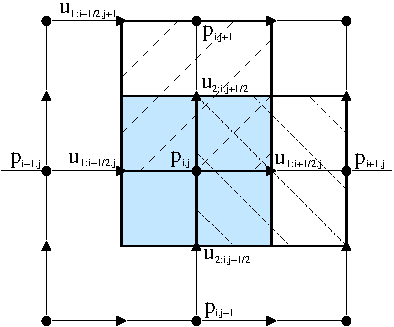
\includegraphics[width=\textwidth]{plots/stag-grid.pdf}
\end{center}
\caption{A 2D schematic of the staggered spatial configuration of the
pressure and velocity variables.
The pressure $p_{i,j}$ is based on the center of its control volume (light colour area);
the horizontal velocity component $u_{1;i+1/2,j}$ is defined in the middle of the
right edge of the pressure control volume and centered on its control volume
(dash-dotted area); the vertical velocity component $u_{2;i,j+1/2}$ is defined in the
middle of the top edge and centered on its corresponding control volume (dashed area).
The volume fraction is defined at the same location as that of the pressure, 
resulting in pressure and density being centered on identical control volumes.  
}
\label{stag-grid}
\end{figure}


To estimate the advecting velocities $u_f^{\textrm{(advecting)}}$ we use a centered scheme.
Consider a face perpendicular to the horizontal direction $1$
\sidenote{
In particular , $f=1-$. 
}
There are two cases, the first corresponding to when 
the advected component is not aligned with the 
face normal, which is the case with $q=2$. 

\marginnote{
The $u_2$ control volume in Fig. \ref{stag-grid} is centered on $i,j+1/2,k$, and face $f=1-$ is then 
centered on $i-1/2,j+1/2,k$. 
}

The advecting velocity  $u_{1-}^{\textrm{(advecting)}}$ 
is not given on this point, therefore it has to be interpolated as - 


\begin{figure}
\begin{center}
    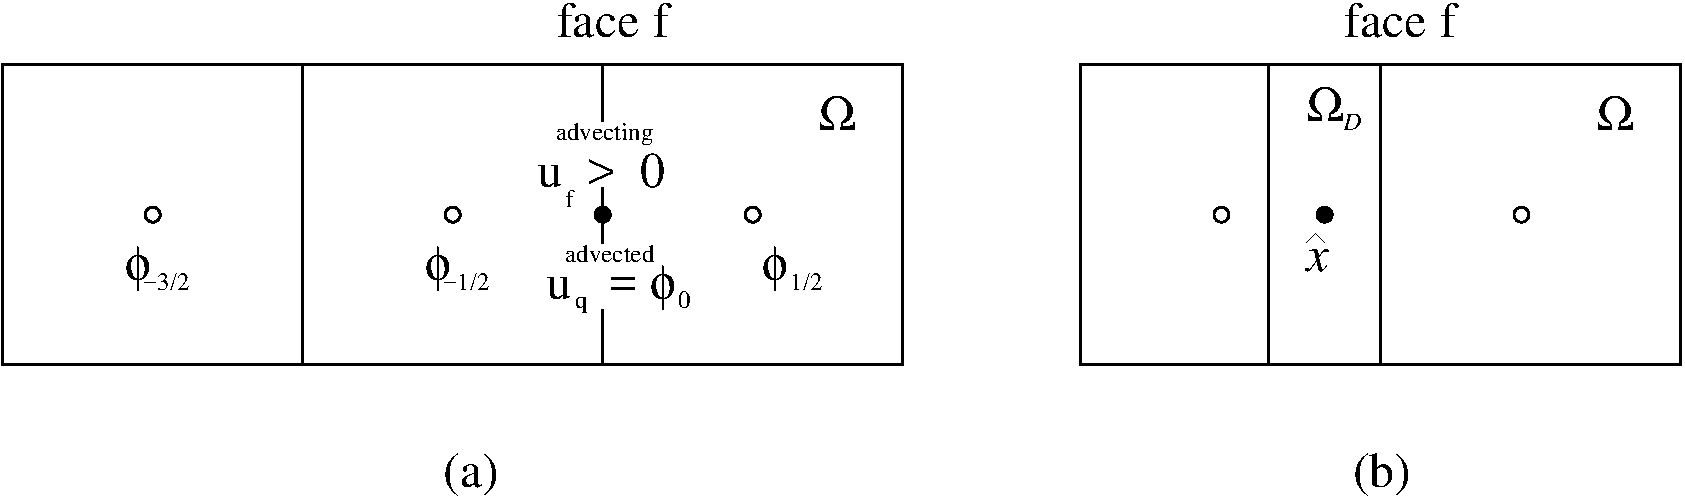
\includegraphics[width=\textwidth]{plots/advect-ed-ing.pdf}
\end{center}
\caption{The reference control volume $\Omega$ for the advected velocity component 
$\phi=u_q$ is shown. A horizontal advection is here considered and both the advecting velocity 
$u_f$ and the advected velocity require an interpolation for their value on the left face 
$f=1-$: (a) the value $\bar u_q = \phi_0$ (full circle) is interpolated 
(see \ref{appendix}) from the values $\phi=u_q$ on the nodes (open circles);
(b) a more sophisticated interpolation predicts the value $\phi(\hat x)$ where $\hat x$ is
at the center of the ``donating'' region $\Omega_D$ (see \ref{appendix}).}
\label{advect-ed-ing-fig}
\end{figure}




\begin{align}
 u_{1;i-1/2,j+1/2,k}^{\textrm{(advecting)}} = \frac12 \big( u_{1;i-1/2,j,k} + u_{1;i-1/2,j+1,k} 
\big) \,
\label{uf2}
\end{align}


In the second case the advected component is aligned with the 
face normal, corresponding to $q=1$. 
\marginnote{
The $u_1$ control volume 
in Fig. \ref{stag-grid} is centered on $i+1/2,j,k$ and face $f=1-$ is then 
centered on $i,j,k$.
}
In this case, the interpolation becomes -  


\begin{align}
	u_{1;i,j,k}^{\textrm{(advecting)}} = \frac12 \big( u_{1;i-1/2,j,k} + u_{1;i+1/2,j,k} \big) \,
\label{uf1} 
\end{align}
 

Thus far, we have covered only interpolations
concerning the ``advecting'' velocity, which is basically
used to compute fluxes of the volume fraction. 
Now we turn our attention to interpolations of the \textit{advected}
velocity $\bar u_{q}$ which appears in \eqref{advect-ed-ing-2}. 
\marginnote{
The interpolants we use in this case are
one-dimensional and operate on the velocities $u_q$, on the center of their 
control volumes, that are regularly spaced on a segment aligned 
with the direction of the advection, that is also perpendicular to face $f$. 
}
In Fig. \ref{advect-ed-ing-fig}, we demonstrate the principle 
behind our interpolation scheme along the horizontal direction $1$, 
with the lighter notation $\phi = u_q$.
The objective is to interpolate the ``advected'' velocity on the left face
of the reference control volume $\Omega$.
In case of advected velocity $u_1$ and the advecting velocity \eqref{uf1} on face
$f=1-$, the relationship with the $\phi$ values in Fig. \ref{advect-ed-ing-fig} is -


\begin{align}
\phi_{-3/2} = u_{1;i-3/2,j,k}, \quad \phi_{-1/2} = u_{1;i-1/2,j,k}, \quad   
\phi_{1/2} = u_{1;i+1/2,j,k}, \;\cdots
\end{align}


whereas in the case of the ``advected'' velocity $u_2$ and the advecting velocity \eqref{uf2},
the relationship turns out to be -


\begin{align}
\phi_{-3/2} = u_{2;i-2,j+1/2,k}, \quad  \phi_{-1/2} = u_{2;i-1,j+1/2,k}, 
\quad  \phi_{1/2} = u_{2;i,j+1/2,k}, \;\cdots
\end{align}

In order to get a prediction of $\phi_0$ on the 
face $f=1-$ in Fig. \ref{advect-ed-ing-fig}
\sidenote{ $\phi_0$ serves as an approximation of 
$\bar u_q$ given in \eqref{barudef}.
}
we use an interpolation function $f$ that computes 
this value as a function of the four nearest points,
and in an upwind manner based on the sign of the 
\textit{advecting} velocity $u_f$. Thus, the interpolation
can be expressed in functional form as - 

\marginnote{
The extension of these approximations to advection along 
the other two directions $q=2,3$ is straightforward. 
}

\begin{align}
\phi_0 = f \left( \phi_{-3/2}, \phi_{-1/2}, \phi_{1/2},\phi_{3/2},\textrm{sign}(u_f) \right)
\label{simpleinterp}
\end{align}


Throughout this body of work, we have extensively tested and used 
two variants of such interpolation functions, the exact implementation 
of which can be found in Appendix A. The interpolation functions are :


\marginnote{The reader can refer to influential works of 
LeVeque \cite{flim_1} and Sweby \cite{flim_2} regaring the role
of non-linear flux limiters such as QUICK, Superbee, WENO/ENO etc 
in the context of numerical methods for hyperbolic conservation laws. 
}

\begin{enumerate}
\item A scheme based on the QUICK 
third order interpolant in the bulk, away from the interface 
and a simple first order upwind flux near the interface. 
\item A scheme based on the Superbee slope limiter \sidecite{roe1985some} for the flux in the 
bulk and a modified Superbee limiter tuned to a shifted interpolation point near the 
interface.  
\end{enumerate}



% ----------------------------------------------------------------------------------------------------------------------


\section{Advection on Staggered Grids}

The development of the consistent transport schemes should be integrated into
the broader context of our numerical algorithm which deals with the 
coupling between the conservative formulation of the 
one-fluid Navier-Stokes equations and the geometric transport of the interface.  
We briefly recapitulate the overall algorithm in operator form as previously described in 
chapter \ref{ch:method}


\marginnote{The superscript $h$ refers to discretization in space, 
and $n$ corresponds to that in time.}


\begin{align}
	C^{n+1} &= C^{n} + \tau L^{h}_{\textrm{vof}}\left( C^{n},\boldsymbol{u}^{n}\right) \\  
	\rho^{n+1}\cdot \boldsymbol{u}^{*} &= \rho^{n}\cdot \boldsymbol{u}^{n} + \tau L^{h}_{\textrm{adv}}\left( C^{n},\boldsymbol{u}^{n} \right) + \nonumber \\
				      & \tau \left[ L^{h}_{\mu}\left(C^{n+1},\boldsymbol{u}^{n}\right) + L^{h}_{\sigma}\left(C^{n+1}\right) + L^{h}_{\textrm{g}}\left(C^{n+1}\right)\right]
\label{global_eqns}
\end{align}


\marginnote{
$L_{\textrm{adv}}$ represents the conservative advection, 
$L_{\mu}$ represents the diffusive forces generated by viscous stresses,
$L_{\sigma}$ represents the capillary forces arising from the surface tension model
and finally $L_{g}$ represents the volumetric (body forces) source term. 
}


In the preceding sections, we have thus far dealt with the 
intricacies concerning the coupling of the VOF advection ($L^{h}_{\textrm{vof}}$)  
with that of the momentum advection ($L^{h}_{\textrm{adv}}$). In this section, we
describe two distinct strategies that we have implemented in order to achieve 
discrete consistency between mass (VOF) and momentum transport, specifically 
in the context of staggered Cartesian grids, with the configuration
already illustrated in Fig. \ref{stag-grid}. 


\subsection*{Shifted Fractions Method}
% algorithm, flow chart , how to reconstruct on shifted grid, lack of conservation 

This strategy tackles the problem of staggered control volumes by reconstructing 
\sidenote{The reconstructions involve geometrical operations, thus are not
easily translated into equations.}
the centered volume fraction field onto the staggered control volumes 
, thereby resulting in a field of \textit{shifted} fractions. 


\begin{figure}
\begin{center}
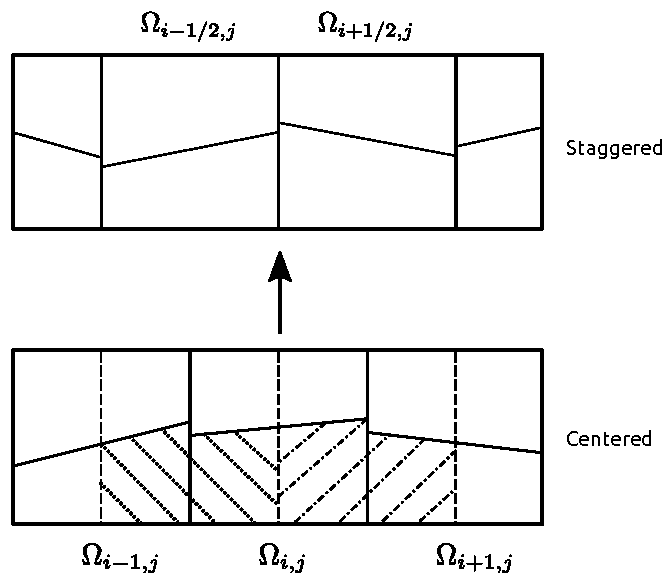
\includegraphics[width=\textwidth]{plots/shifted_fractions.pdf}
\end{center}
\caption{A 2D schematic of the reconstruction procedure 
used in the \textit{shifted fractions} method. 
In this case, advection of the horizontal component of momentum is considered.
The half-fractions from the centered control volumes 
$\Omega_{i,j}$ and $\Omega_{i+1,j}$ (dash-dotted area) are added together
to obtain the volume fraction in the shifted (staggered) volume $\Omega_{i+1/2,j}$.
Similarly, the half-fractions from $\Omega_{i-1,j}$ and $\Omega_{i,j}$ (dotted area)
are combined to obtain the volume fraction $\Omega_{i-1/2,j}$.
Once this horizontally shifted volume fraction field is reconstructed, 
the corresponding density, momentum and ``advected'' velocity fields can be 
computed in order to carry out consistent transport of mass and momentum
on this staggered configuration. 
}
\label{shift_frac}
\end{figure}


A 2D schematic of this reconstruction procedure is given in Fig. \ref{shift_frac} 
, considering the advection of the horizontal component of momentum. 
At the beginning of the operations summarized by $L_{\textrm{adv}}$, 
each velocity (momentum) control volume overlaps two pressure/VOF (centered)
control volumes i.e.  $\Omega_{i+1/2,j}$ overlaps $\Omega_{i,j}$ and $\Omega_{i+1,j}$
Therefore, the two half-fractions from $\Omega_{i,j}$ and $\Omega_{i+1,j}$ are 
added together to obtain an estimate
\sidenote{These estimations utilize the set of geometric operations
that are used in the reconstruction of the interface and fluxed volumes.
The reader can refer to chapter \ref{ch:method} for a brief reminder.}
of the shifted fraction $C_{i+1/2,j}$ in $\Omega_{i+1/2,j}$. 
Once this key reconstruction step is carried out, the mass and momentum
fields, as well as their corresponding fluxes can all be derived using the information
from the shifted volume fraction field. These operations performed at each time step
are summarized in the following steps : 


\begin{enumerate}

\item Interface reconstruction at time $t_n$ using data $C^{n}$.
        
	\marginnote{$q=1,2,3$ is the component index, 
	e.g $\rho_1$ in $\Omega_{i+1/2,j,k}$ for the 
	horizontal momentum component $\rho_1 u_1$.
	}

\item Computation of half-fractions as shown in Fig. \ref{shift_frac},
	in order to obtain the ``shifted'' fraction field $C^{n}_q$ and $\rho^{n}_q$
	in the staggered control volumes.

\item Computation of all three momentum components $(\rho_q u_q)^{n}$
	at $t_n$.
	\marginnote{ The fluxes of momentum are derived from those of mass
		using the relation \eqref{frou} ,
		which in turn are obtained in a consistent fashion from 
		the fluxes corresponding to `shifted' volume fraction field.}

\item Advection of all three momentum components along one coordinate direction,
	say $x$ direction, using \eqref{sumfmom2} to obtain the updated momentum components
	$(\rho_q u_q)^{n,1}$ after the first substep.

\item Advection of the ``shifted'' density field $\rho^{n}_q$ on the staggered volumes 
	using VOF consistent advection, along the $x$ direction in order to
	 obtain the updated volume fractions after the first substep.

\item Extraction of the provisional velocity components 
	\sidenote{These provisional velocities are required
		to compute the ``advected'' velocities using 
		the non-linear flux limiters, as described in \eqref{advect-ed-ing-2}.}
	$u_q^{n,1}$ after the first substep, i.e. $u_q^{n,1} = (\rho_q u_q)^{n,1}/\rho_q^{n,1}$.

\item The above operations are repeated for the different momentum components, shifted
volume fractions and densities, and velocity components for the next two substeps
with split advections along the $y$ and $z$ directions.
\sidenote{At each time step, the sequence $x, y, z$ is permuted, in order to avoid 
any systematic biases in error propagation.}
Finally, we obtain $(\rho_q u_q)^{n+1} = (\rho_q u_q)^{n,3}$ and
$\tilde \rho_q^{n+1} = \rho_q^{n,3}$. 

\item In parallel, the centered volume fraction field $C^{n}$ 
	is advected in order to obtain $C^{n+1} = C^{n,3}$ using the VOF advection method. 

\end{enumerate}


\begin{figure}
\begin{center}
    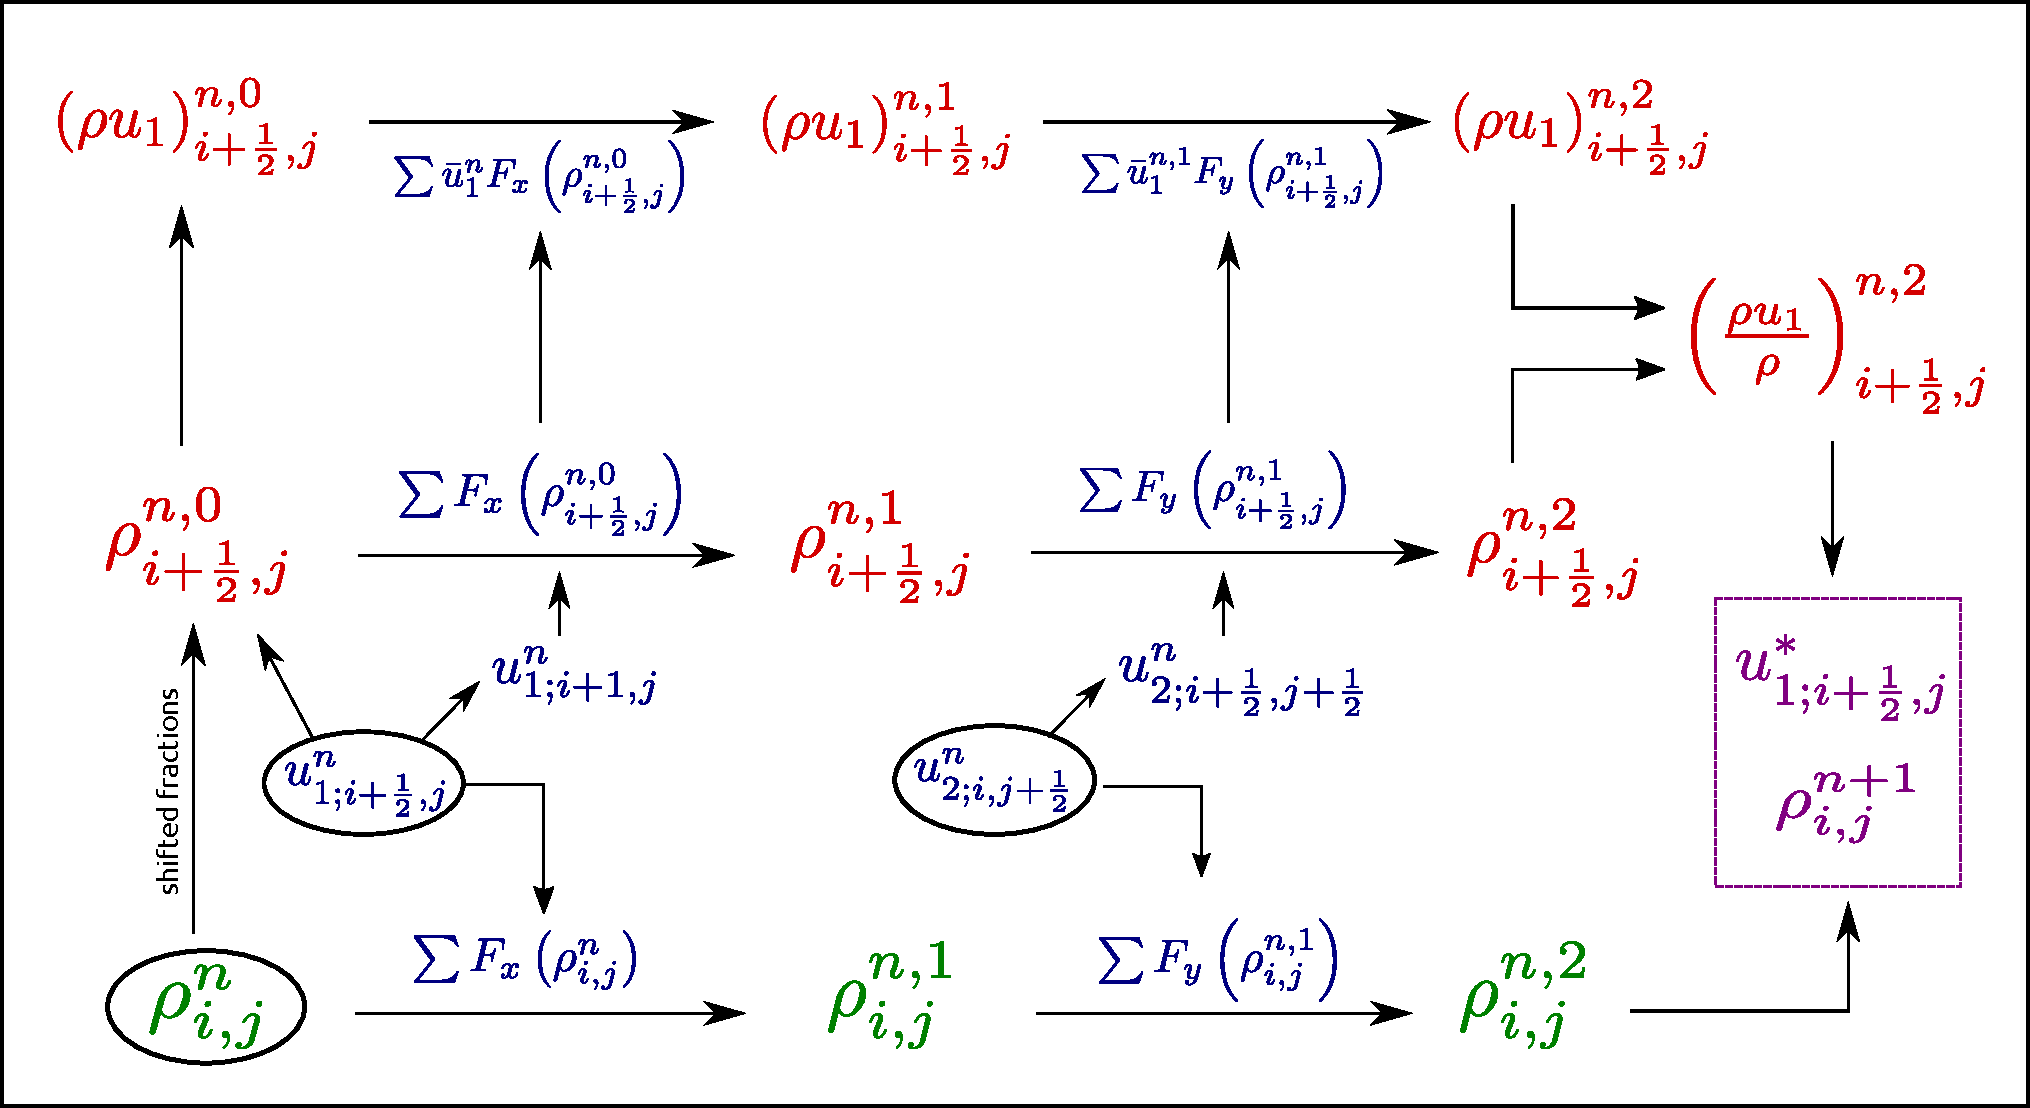
\includegraphics[width=\textwidth]{plots/momcons_diagram_daniel.pdf}
\end{center}
\caption{A bird's eye view of the \textit{shifted fractions} method,
highlighting the operations performed at each time step. 
This method achieves consistency in the discrete transport 
of mass and momentum on the staggered control volumes.
In the interest of brevity, we present a 2D case for the
density on the grid $i,j$ and horizontal velocity $u_1$ on the staggered grid $i+1/2,j$.
The evolution of the velocity component $u_2$ on the staggered grid $i,j+1/2$ is similar.
The initial variables $\rho^n$, $u_1^n$, $u_2^n$ are inside the ellipses. The interpolated
``advecting'' components $u_1$ and $u_2$ have superscript $n$. The shifted density $\rho^{n,0}$
is constructed with the shifted fractions of $C$ to initialize the momentum component
$(\rho u_1)^{n,0}$. The first split advection is along the $x$ direction  to 
variables with superscript $n,1$, the second one is along the $y$ direction to
variables with superscript $n,2$. The updated density is $\rho^{n,2}=\rho^{n+1}$
while the horizontal velocity $u_1^{n,2}=u_1^{*}$ enters the RHS of the Poisson-like
equation \ref{poisson}. }
\label{momcons_daniel}
\end{figure}


An important point to note from the above algorithm is that 
the advected velocity components $u_q$ are updated at each substep,
while the advecting velocities $u_f$ are interpolated from the initial
velocity field $\boldsymbol{u}^n$ at time $t_n$. 
The shifted fractions of Fig. \ref{shift_frac}
are computed using routines that are already part of our
geometrical toolbox, used primarily in flux computation. 


In essence, we have a consistent transport of density (mass)
and momentum on the staggered grids, while simultaneously 
carrying out advection of the volume fraction field on the centered grid. 
\marginnote{
A naive attempt to achieve momentum conservation could entail always using the 
shifted fields $C^{n}_{q}$ and evolve them by the VOF method on the staggered cells. 
Such an approach would render the scheme conservative, but would result in the  
independent evolution of the three staggered grids, eventually leading to divergence.
}
As a consequence, the momentum components $(\rho_q u_q)^{n+1}$ 
(at time step $t_{n+1}$) that are derived from the 
corresponding ``shifted'' volume fractions $C^{n+1}_q$ 
and densities $\rho^{n+1}_q$  (obtained from $C^{n+1}$)
are different from the densities $\tilde \rho_q^{n+1} = \rho_q^{n,3}$
, which were computed during the previous time step 
by directly advecting the ``shifted'' volume fractions $C^{n}_q$. 
The origin of this discrepancy is the approximate nature of the  
linear reconstruction of the interfaces, which is not 
even continuous on the boundary of its control volume.
Therefore, this implies that the momentum is not exactly
conserved between two time steps, even though the Weymouth-Yue method
ensures conservative transport of the momentum on the staggered control volumes. 


%--------------------------------------------------------------------------------------


\subsection*{Sub-Grid Method}

In this strategy, the difficulty associated with consistent 
transport on staggered control volumes is resolved by advecting  
the volume fraction (mass) on a twice finer grid 
\sidenote{
The grid is twice as fine when compared to the control volume for momentum.
} , very much in the spirit of Rudman's \cite{rudman1998volume} original work. 

The primary motivation regarding the development of this 
method is the issue of conservation (lack of) concerning 
the discrete transport of momentum in case of the shifted fractions method.     
Basically, the issue arises quite simply due to the fact that the volume fraction 
$C^{n+1}$ used to construct the staggered momentum field at the start of a 
new time step is \textit{not} the identical to that which is obtained 
via advection on the staggered control volumes itself ($C_{q}^{n+1}$). 
\sidenote{
In the shifted fractions method, flux computations on the staggered 
cells necessitate another round of interfacial reconstructions based on the shifted 
volume fraction field, whereas the sub-grid volume fraction information enables one
to circumvent the reconstructions and obtain the fluxes directly using simple surface integrals.
}
The sub-grid method is able to evade these complications that arise due to
the parallel evolution of two different volume fraction fields by conducting 
volume fraction on solely on the twice refined grid.  
An additional advantage of the having the sub-grid volume fraction field is that 
it facilitates a more `natural' computation of not only the staggered 
volume fraction field $C^{n+1}_q$, but more importantly its fluxes. 
This method is currently only compatible with the implicit fluxes 
computed in the Weymouth-Yue VOF advection method. 

Considering the overall approach, the \textit{key differences} between our 
present algorithm and the implementations in the 
original works of Rudman and Weymouth-Yue are : 

\begin{description}
	\item[Rudman (1998)\cite{rudman1998volume} ] The use of a conservative geometrical 
		mass (volume fraction) transport framework instead of an algebraic one in 
		the original method, which is applied to sub-grid volume fraction field.  
	\item[Weymouth \& Yue (2010) \cite{wy}] The extension of the 
		original method for conservative direction-split mass transport to the momentum field, 
		culminating in the discrete consistency between mass 
		momentum transport in the context of staggered Cartesian grids in 3D. 
\end{description}


\subsubsection*{Spatial Configuration : Coarse \& Sub-Grid Variables}

\begin{figure}[h!]
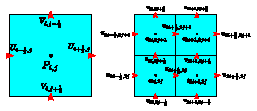
\includegraphics[width = \textwidth]{plots/sub_grid.pdf} 
\centering
\caption{A 2D schematic of the arrangement of primary variables 
on the coarse and sub-grid levels. 
The control volume is decomposed into the two figures, the one
on the left corresponding to the coarse grid variables, while the 
one on the right corresponding to the sub-grid. 
Superposition of these two figures, one on top of each other,
represent the spatial relationships between the two sets of variables.
The velocities on the sub-grid level are simple first 
or zeroth order interpolations of the coarse grid velocities.
}
\label{sub_grid}
\end{figure}

To start, we describe the spatial orientation of the different 
variables on the two refinement levels of the grid.   
\marginnote{The notations for the variables are slightly
different that those used in the previous sections (Fig. \ref{stag-grid}.) 
The velocity component in the horizontal and vertical directions 
are now denoted as $U$ and $V$ respectively, and the pressure by $p$. 
}
At the coarse grid level, the pressure and velocity fields are 
defined in a staggered configuration, with pressures at the cell 
centers (centroids in 3D) and velocities on the cell face centers. 
In Fig. \ref{sub_grid}, we demonstrate the arrangement of variables, 
which one can easily extrapolate to 3D during implementation, 
but for the sake of clarity we illustrate its 2D equivalent. 
The volume fraction $C$ 
\sidenote{ The volume fraction field $C$ is denoted as $c$ in Fig. \ref{sub_grid}. 
} is only defined on a grid that is twice as fine than 
that of the pressure/velocity grid, which we refer to as the sub-grid. 
Therefore in 3D, each cubic control volume is divided into eight constituent 
smaller cubic volumes at the centroids of which, the volume fraction field is centered. 


\subsubsection*{Multiscale Coupling : Restriction \& Prolongation Operations}

As is paradigmatic for dual-grid methods in the context of 
Navier-Stokes solvers, we carry out mass transport 
at the sub-grid level, and momentum transport at the coarse level. 
In pressure-projection based methods such as ours, the predominant 
bottleneck in terms of computational speed is the 
iterative solution to the discrete Poisson equation. 
\sidenote{
The problem size of such elliptical 
partial differential equations is governed by 
the number of cells/points discretizing the velocity (or pressure) field. 
If we choose to solve the problem on a mesh with
twice the resolution in 3D, that would lead to an 8 fold increase 
in the problem size for the discrete pressure-Poisson problem.   
}
Therefore, solving the mass advection equation on the fine grid 
allows us not only to obtain more accurate solutions to the flow physics 
involved, but also enables us to avoid the significantly higher  
computational costs associated with solving a Poisson problem 
at a twice finer resolution.  

\paragraph{\textbf{Prolongation}}

In order to advect the volume fraction at the sub-grid level, 
we need to reconstruct a velocity field at that level of resolution using 
information from the coarse grid velocity field.
\marginnote{ 
The prolongation operator has to be used at the start of each new time step,
in order to compute the sub-grid velocity field. 
}
In order to achieve this, we have implemented a prolongation operator 
which asserts the following relations between the velocities on the two refinement levels  

\begin{align}
  	  u_{2i-\frac{1}{2},2j} = u_{2i-\frac{1}{2},2j+1} &= U_{i-\frac{1}{2},j} \\ 
            u_{2i+\frac{3}{2},2j} = u_{2i+\frac{3}{2},2j+1} &= U_{i+\frac{1}{2},j} \\ 
  	  u_{2i+\frac{1}{2},2j} = u_{2i+\frac{1}{2},2j+1} &= \left(U_{i+\frac{1}{2},j} + U_{i-\frac{1}{2},j}\right) / 2 \\
  	  v_{2i,2j-\frac{1}{2}} = v_{2i+1,2j-\frac{1}{2}} &= V_{i,j+\frac{1}{2}} \\ 
            v_{2i,2j+\frac{3}{2}} = v_{2i+1,2j+\frac{3}{2}} &= V_{i,j-\frac{1}{2}} \\
  	  v_{2i,2j+\frac{1}{2}} = v_{2i+1,2j+\frac{1}{2}} &= \left(V_{i,j+\frac{1}{2}} + V_{i,j-\frac{1}{2}}\right) / 2 
\end{align}


The notations in the above equations refer to the description 
of the coarse and sub-grid variables in Fig. \ref{sub_grid}. 
The first-order interpolation applied to the coarse grid 
velocity field ensures discrete incompressibility 
\sidenote{This is a direct consequence of the solenoidal 
nature of the coarse grid velocity field.
}
at the sub-grid level.
The choice of interpolation order used in the  prolongation operator 
is identical to that of the originial method of Rudman (\cite{rudman1998volume}). 
In the current version of the sub-grid method, we have chosen to eschew the added 
complexity of solving local Poisson problems 
\sidenote{
The use of higher order interpolation schemes would necessitate 
finding the solutions of local Poisson problems, in order to 
render the sub-grid velocity field discretely divergence-free. 
}
through our prolongation operators, therefore sticking with 
the much simpler Rudman inspired interpolations. 


\paragraph{\textbf{Restriction}}


\begin{figure}[h!]
\centering
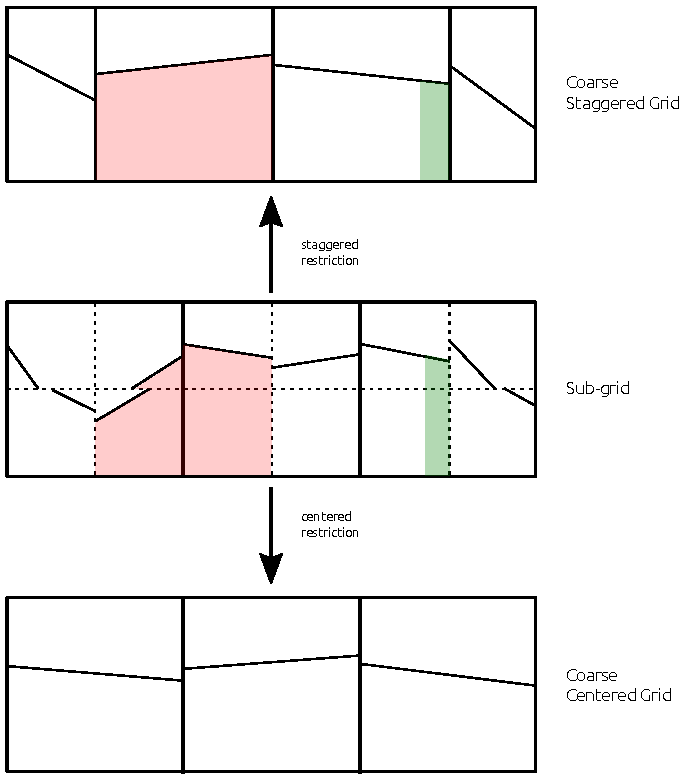
\includegraphics[width = \textwidth]{plots/subgrid_restriction.pdf}
\caption{A 2D illustration of the restriction operations involved
	between the different grid resolutions, where the sub-grid 
	grid boundaries are denoted by the dashed lines, 
	and that of the overlapping coarse grid by solid lines. 
	Restriction operations in the form of simple volume integrals
	are performed on the sub-grid volume fraction in order
	to compute the staggered and centered volume fraction 
	fields at the coarse grid level. 
	Restriction operators in the form of surface integrals 
	are also performed in order to compute the volume fluxes
	at the boundaries of the coarse staggered control volumes.
	The red shaded areas correspond to the volume fractions, 
	whereas the green shaded area corresponds to that of volume fluxes.
        The interface segments as depicted at the coarse grid level 
	are just for purpose of illustration, and are not
	`reconstructed'. Unlike the shifted fractions method, the 
	interfacial reconstructions on the staggered volumes are not 
	necessary, due to the fact that sub-grid volume fluxes are 
	simply combined to compute the staggered fluxes.  
	}
\label{restrict}
\end{figure}


In order to compute the required density and momentum fields
on the staggered grid (coarse level), we implement restriction operators
that use information from the sub-grid volume fraction field.  
\marginnote{
The restriction operators work in an identical manner as in 
Rudman (\cite{rudman1998volume}), which are nothing but simple volume 
integrals of the sub-grid field mapped onto the domains corresponding 
to the coarse grid control volumes. 
}
In Fig. \ref{restrict}, we demonstrate the different 
mappings between the two grid levels, which essentially boils down 
to volume integrals for the centered fields, and surface integrals 
for their corresponding fluxes.
A description of the different functions performed by the restriction 
operator is as follows : 

\begin{itemize}
	\item \textit{Fine Grid $\longmapsto$ Coarse Staggered Grid}
          
	  \begin{description}
		  \item[Density \& Momentum] The sub-grid volume fraction field
			  is restricted to obtain a staggered density field at the 
			  coarse grid level (see Fig. \ref{restrict}), which on combining with 
			  the appropriate component of the velocity field 
			  produces the staggered momentum field.    
		  \item[Fluxes] The geometric fluxes from the sub-grid volume fraction 
			field are restricted in order to obtain coarse grid fluxes for the 
			 corresponding staggered volumes, which on combining with 
			  relation \eqref{frou} gives us the corresponding momentum fluxes.   
	  \end{description}

  \item \textit{Fine Grid $\longmapsto$ Coarse Centered Grid}

          \begin{description}
		  \item[Density \& Viscosity] The sub-grid volume fraction field is 
			  restricted to compute a centered volume fraction field at the 
			  coarse grid level, which is subsequently used to derive the  
			  centered density and viscosity fields at the coarse grid level.   
	  \end{description}

\end{itemize}


\subsubsection*{Algorithm}

To summarize the operations performed at each time step
pertaining to the advection operator in our one-fluid Navier-Stokes framework, 
we present Fig. \ref{momcons_sagar}, which illustrates a 2D version 
of the sub-grid method that ensures consistent and conservative 
mass-momentum transport, highlighting the interactions between the 
variables defined on the different grids. The algorithm is also
summarized in the following steps, corresponding to a 2D setup : 


\begin{figure}
\centering
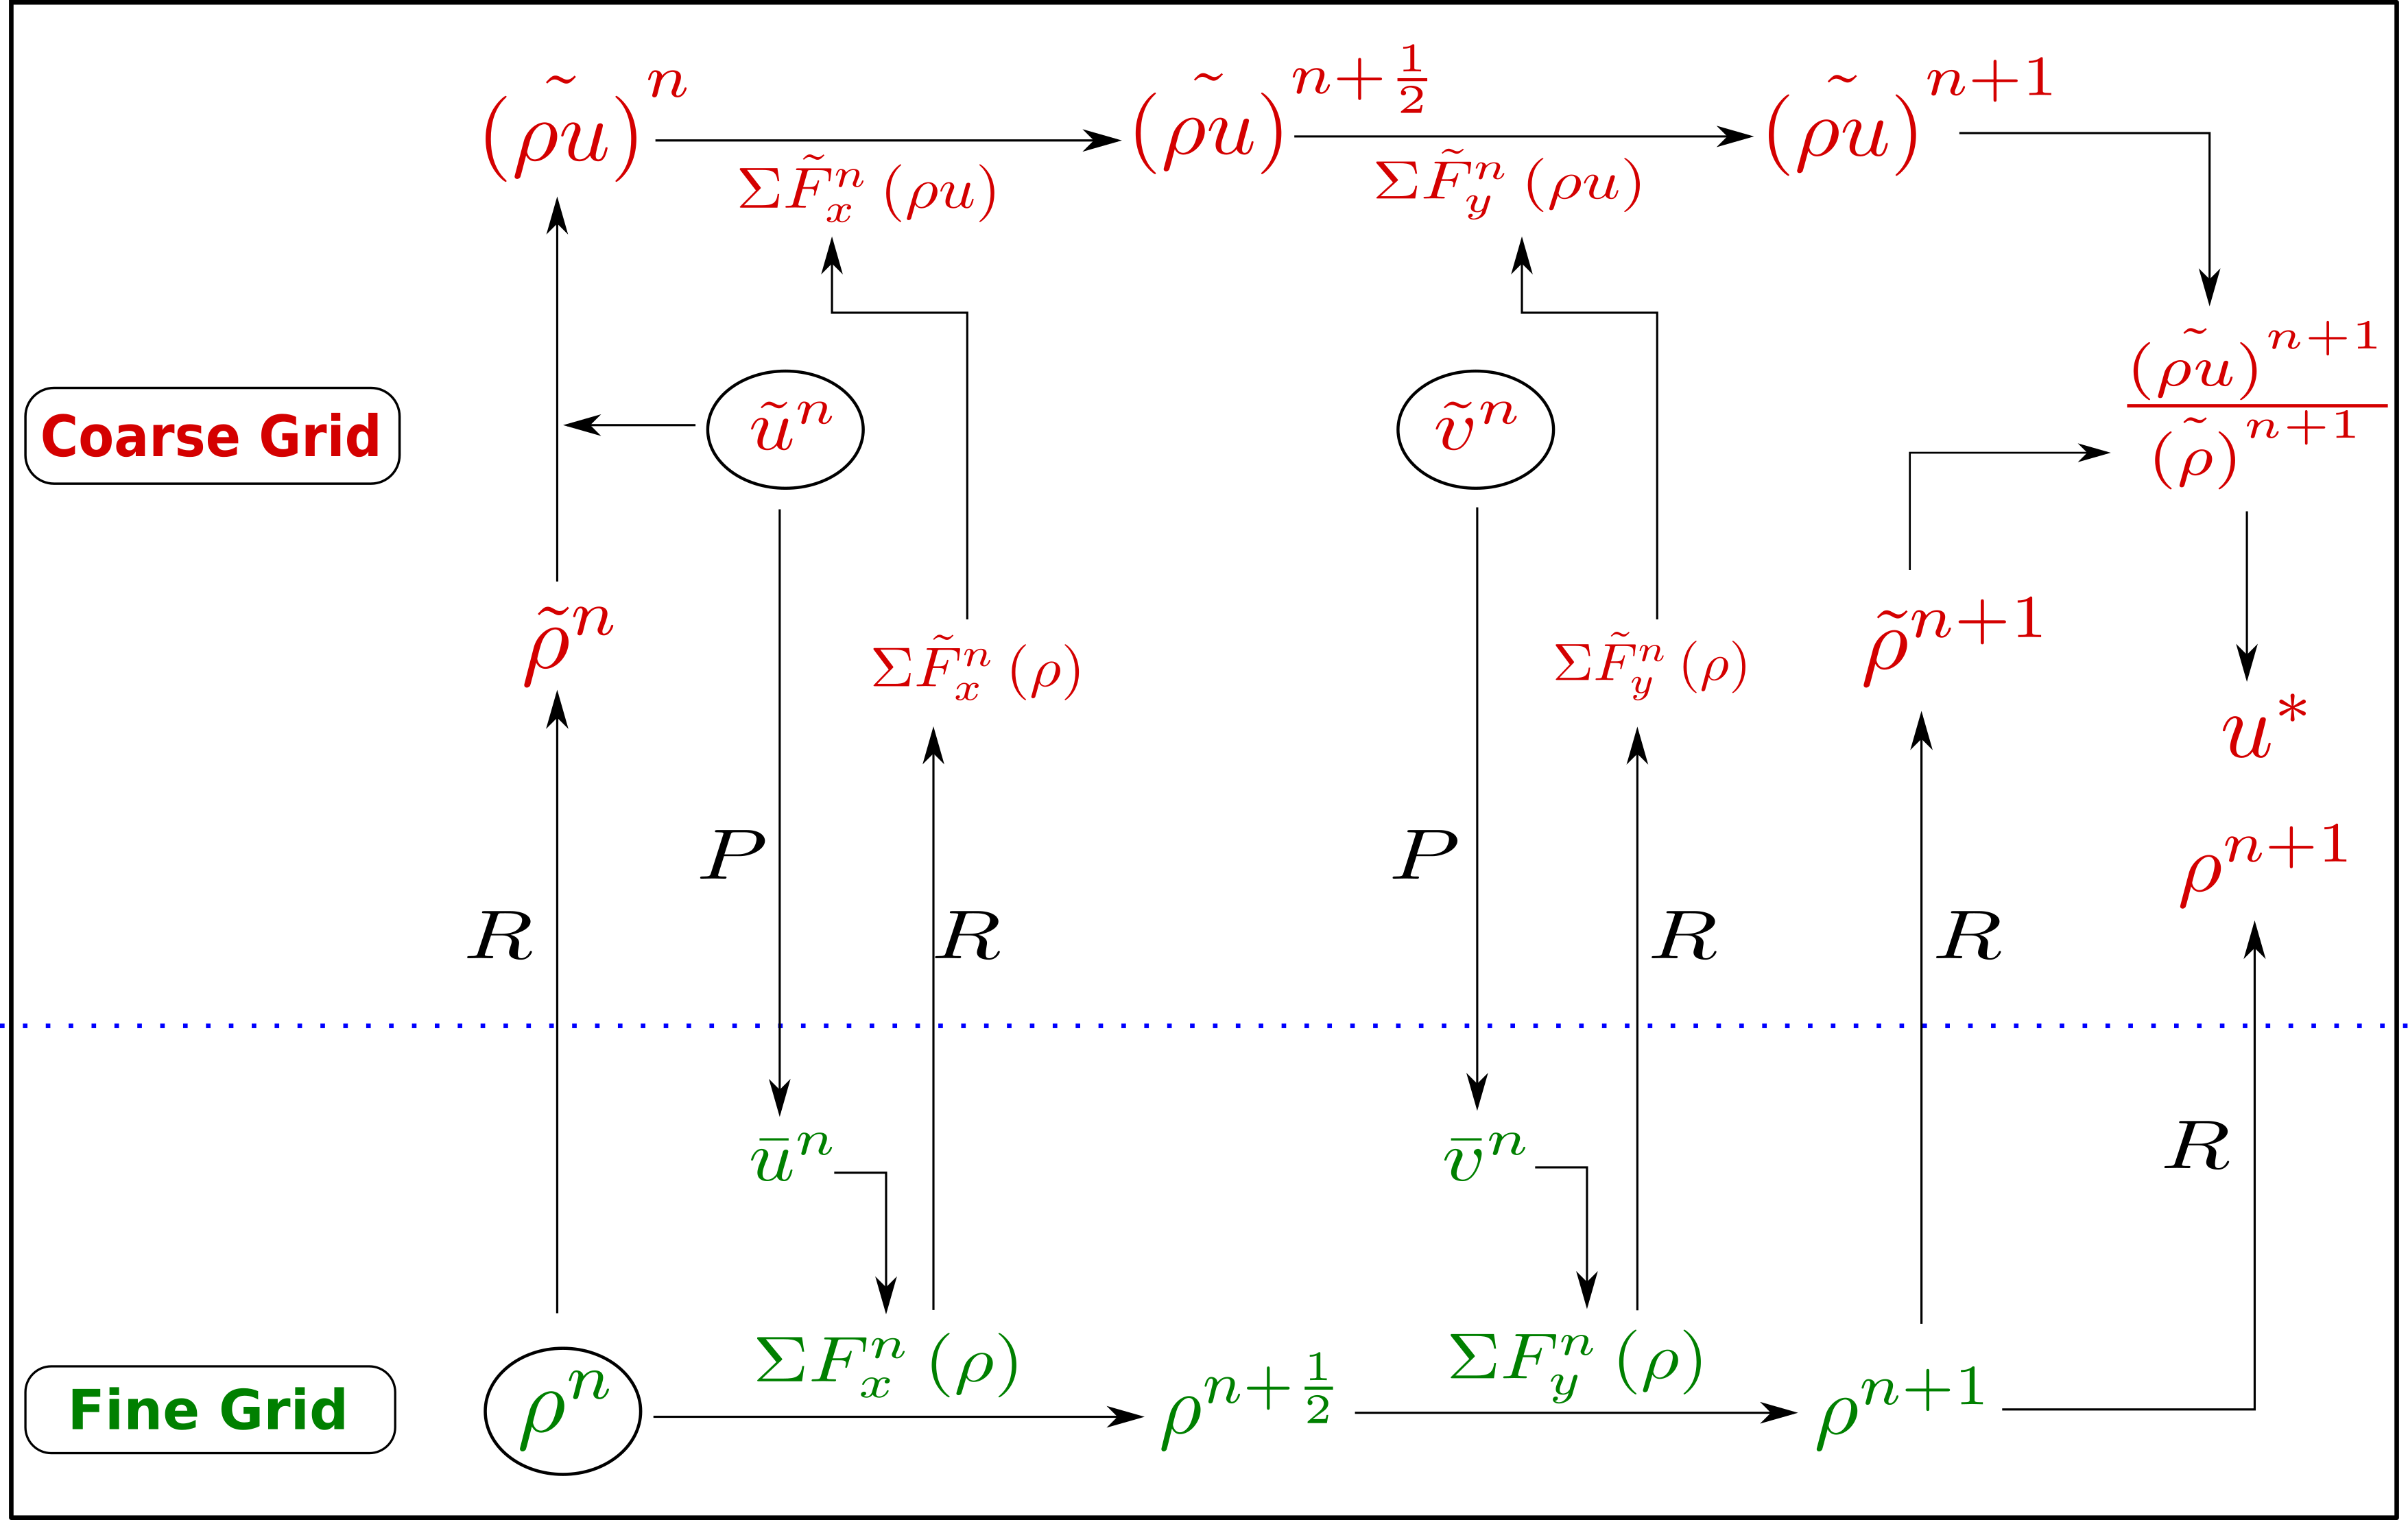
\includegraphics[width = \textwidth]{plots/momcons_sagar.png}
\caption{A bird's eye view of the \textit{sub-grid} method,
highlighting the operations performed at each time step. 
and additionally ensures conservation of momentum.
For sake of clarity, present a 2D case for the
density on the grid $i,j$ and horizontal velocity $\tilde{u}$ 
on the staggered grid $i+1/2,j$.
The variables in red are all defined on the coarse level, 
and those in green are at the sub-grid level. 
The operators $R$ and $P$ denote the restriction and 
prolongation operations respectively.
The 'tilde' on top of the variables (e.g. $\tilde{\rho}^{n} $) are 
used to convery that the variables are centered on the  
staggered control volumes at the coarse grid level, whereas the 'bar' 
on top conveys that the variables are staggered with respect to the sub-grid. 
The starting variables are enclosed in elliptical borders, 
and the variables at the end of the direction-split 
integrations are $u^{*}$ and $\rho^{n+1}$,
where $u^{*}$ is subsequently fed into the RHS of the Poisson problem. 
}
\label{momcons_sagar}
\end{figure}



\begin{enumerate}

\item Interface reconstruction at time $t_n$, at the sub-grid level,
	using data $c^{n}$.
        
	\marginnote{$q=1,2$ is the component index, 
	e.g $\rho_1$ in $\Omega_{i+1/2,j}$ for the 
	horizontal momentum component $\rho_1 u_1$.
	}

\item Restriction of the sub-grid volume fraction in order     
	to compute the ``shifted'' fraction fields $C^{n}_q$ and $\rho^{n}_q$
	in the staggered control volumes.

\item Computation of all momentum components $(\rho_q u_q)^{n}$
	at $t_n$.
	\marginnote{ The fluxes of momentum are derived from those of mass
		using the relation \eqref{frou} ,
		which in turn are obtained via restriction operations applied 
		to the sub-grid volume fraction fluxes. 
		}

\item Advection of the sub-grid volume fraction $c^n$ along one coordinate direction, 
	say $x$ direction, to obtain $c^{n + \frac{1}{2}}$ , using the Weymouth-Yue explicit advection method.  
	
\item Advection of all momentum components along the $x$ direction, 
	in sync with the sub-grid VOF advection, 
	using \eqref{sumfmom2} to obtain the updated momentum components
		$(\rho_q u_q)^{n + \frac{1}{2}}$ after the first substep.

\item Restriction of the sub-grid field $c^{n + \frac{1}{2}}$ as shown in Fig. \ref{restrict}
	, in order to compute the ``shifted'' density field $\rho^{n + \frac{1}{2}}_q$ on the staggered volumes. 

\item Extraction of the provisional velocity components 
	\sidenote{These provisional velocities are required
		to compute the ``advected'' velocities using 
		the non-linear flux limiters, as described in \eqref{advect-ed-ing-2}.}
		$u_q^{n + \frac{1}{2}}$ after the first substep, 
		i.e. $u_q^{n + \frac{1}{2}} = (\rho_q u_q)^{n + \frac{1}{2}}/\rho_q^{n + \frac{1}{2}}$.

\item The above operations are repeated for the different momentum components,
	in sync with the direction-split advection of the sub-grid volume fraction
	along the remaining direction. 
\sidenote{At each time step, the sequence $x, y$ is permuted, in order to avoid 
any systematic biases in error propagation.}
Finally, we obtain $u_q^{*} = (\rho_q u_q)^{n + 1}/\rho_q^{n + 1}$ on the staggered grid.

\item In parallel, the updated centered volume fraction field $C^{n+1}$ is obtained  
	at the coase grid level, by applying the restriction operator 
	on the updated sub-grid volume fraction $c^{n+1}$. 

\end{enumerate}

The resulting method not only maintains discrete consistency between
mass and momentum transport on the staggered grid, but also ensures that
the transport of momentum is consistent in 3D.
The other time-split terms in equation (\ref{global_eqns}) 
that arise from the source term discretizations, as well 
as the terms in the projection step \eqref{ufinal} are solved in 
a standard non-conservative way. 
The density on the faces of the central cells 
are estimated using the restriction operations
\marginnote{
Generally, the face-centered density field 
is estimated using a simple average i.e. $\rho_{i+1/2,j,k} = (\rho_{i,j,k} + \rho_{i+1,j,k})/2$. 
}
described previously, with these densities appearing 
via the $ 1 / \rho_q $ pre-factor in front of all
the different source terms. Additionally, the sub-grid volume fraction
can be used to get better estimates of the curvature field, which
itself if defined on the staggered control volumes. At the time of writing, 
two different approaches are being developed and tested in order to 
get more accurate curvature fields. 

In the following chapter, we shall take a look at some performance 
aspects of these mass-momentum consistent methods,
using both quantitative and qualitative comparisons. 



